\documentclass[11pt,a4paper]{article}
\usepackage[a4paper,margin=0.85in]{geometry}
\usepackage[T1]{fontenc}
\usepackage{lmodern}
\usepackage{microtype}
\usepackage{parskip}
\usepackage{graphicx}
\usepackage{array}
\usepackage{hyperref}
\usepackage{xcolor}
\usepackage{enumitem}

\definecolor{accent}{HTML}{17365D}
\hypersetup{colorlinks=true,urlcolor=accent,pdftitle={Zhongli Wang - UBS Cover Letter},pdfauthor={Zhongli Wang}}
\pagestyle{empty}
\setlist[itemize]{leftmargin=1.35em,nosep,itemsep=2pt,topsep=3pt}

\begin{document}

% Title page
\begin{center}
    {\Large \textbf{Job Application}}\\[2.2cm]
    {\Huge \textbf{Zhongli Wang}}\\[0.4cm]
    {\LARGE Application for AI Algo Quant Trader}\\[0.15cm]
    {\large UBS Global Markets, Hong Kong}
\end{center}

\vspace{0.55cm}

\begin{center}
    \IfFileExists{../zhongli-wang-profile.jpg}{
        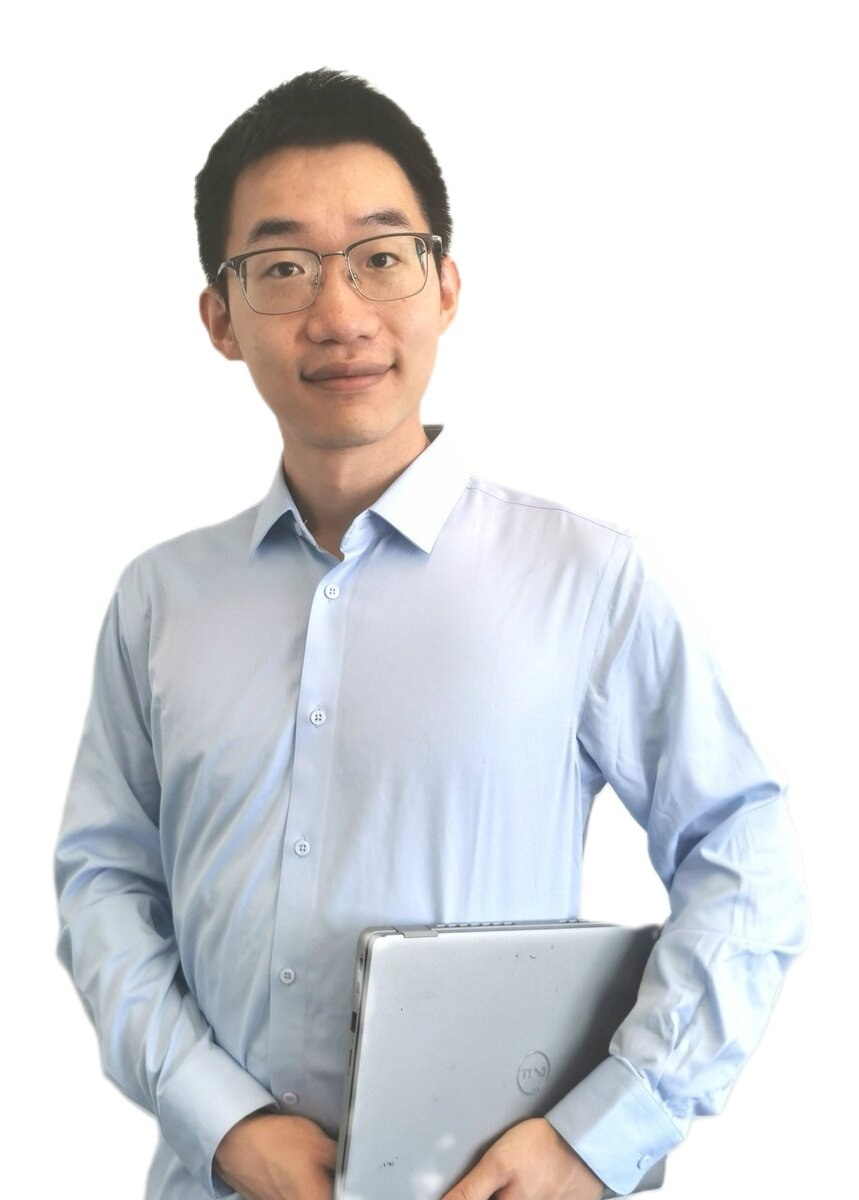
\includegraphics[
            width=0.55\textwidth,
            height=0.43\textheight,
            keepaspectratio
        ]{../zhongli-wang-profile.jpg}
    }{}
\end{center}

\vspace{0.55cm}

\begin{center}
\renewcommand{\arraystretch}{1.35}
\begin{tabular}{>{\bfseries}p{4.2cm} p{8.5cm}}
Address: & Bielefeld, Germany \\
Number: & +49 160 9541 6015 \\
Email: & nkwangzhongli@gmail.com \\
% Reference: & 345113BR \\
\end{tabular}
\end{center}

\newpage

\begin{flushright}
Zhongli Wang\\
Bielefeld, Germany\\
\href{mailto:nkwangzhongli@gmail.com}{nkwangzhongli@gmail.com}\\
+49 160 95416015
\end{flushright}

\vspace{0.15cm}
\today

\vspace{0.15cm}
\noindent UBS Recruiting Team\\
UBS Business Solutions SA

\vspace{0.2cm}
\noindent\textbf{Application for AI Algo Quant Trader, Job Reference 345113BR}

\vspace{0.12cm}
\noindent Dear UBS Recruiting Team,

I recently defended my PhD in Economics at Bielefeld University and hold an MA in Business \& Economics with a major in Banking \& Finance and a minor in Data Science. 
My work combines computational economics, machine learning, financial-data analysis, and AI research workflows, providing a strong foundation for quantitative research in electronic trading.

The role's focus on taking ideas from data and research through rigorous validation particularly matches how I work. 
In my doctoral research, I design computational models, prepare financial data, compare estimation approaches, conduct sensitivity and robustness checks, and communicate findings to international academic and business audiences. My relevant experience includes:

\begin{itemize}
    \item \textbf{Quantitative research:} Building agent-based and statistical models of strategic firm behaviour, market dynamics, and changing economic environments.
    \item \textbf{Machine learning and financial data:} Developing and comparing XGBoost, Random Forest, and neural-network models for financial fraud detection using accounting and market indicators.
    \item \textbf{Python and AI implementation:} Using Python, pandas, NumPy, scikit-learn, and Microsoft AutoGen to build reproducible analysis and end-to-end agentic research workflows.
    \item \textbf{Research ownership and collaboration:} Originating research questions, challenging modelling assumptions, documenting limitations, and working with economists and software engineers to communicate technical results clearly.
\end{itemize}

My background in quantitative economics has trained me to reason carefully about noisy data, model risk, overfitting, changing regimes, 
and the connection between assumptions and measurable outcomes. 
I would bring that discipline, together with strong financial-domain knowledge and a collaborative working style, to research on pricing, execution, liquidity, and automated risk management.

I would welcome the opportunity to discuss how my quantitative research and AI experience could contribute to UBS's electronic trading team in Hong Kong. Thank you so much for your consideration!

\vspace{0.15cm}
\noindent Kind regards,\\[0.05cm]
\vspace{0.1cm}
\noindent
\includegraphics[width=2.7cm,keepaspectratio]{../Wang-sig.jpg}

\noindent Zhongli Wang

\end{document}
